% !TEX root = ../main.tex

\clearpage
% Source PDF page 49.
\section{第十一章\quad 奶科学简介}

在奶蛙的热潮下，各个领域纷纷乱入奶蛙，形成了看似一本正经实则奇异搞笑的奶科学。本章将对几个领域形成的奶科学进行简单介绍。

\subsection{一、奶数学}

奶数学，顾名思义，就是用各种数学的方式表现出奶蛙。在数学分析和工程领域，傅里叶变换能够将一个复杂的图形用三角函数无限逼近模拟。因此，许多大学生使用傅里叶级数来绘制奶蛙。~(见\figref{fig:11-1})

% !TEX root = ../../main.tex
\begin{figure}[H]
  \centering
  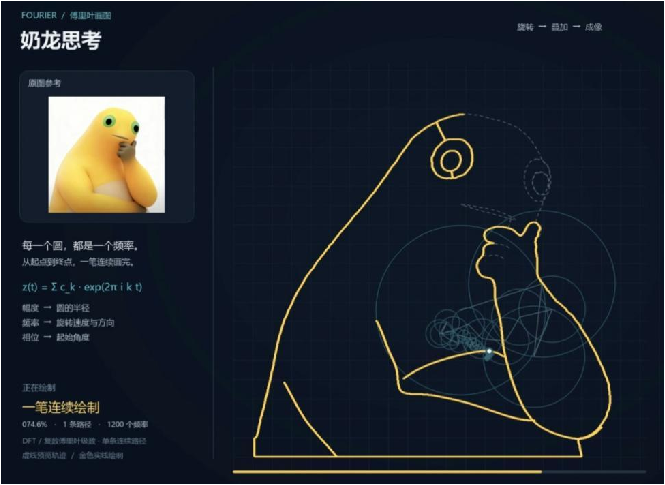
\includegraphics[width=271.15bp,height=0.76\textheight,keepaspectratio]{figures/chapter11/figure11_1.pdf}
  \renewcommand{\thefigure}{11.1}
  \caption{使用傅里叶级数一笔绘制思考奶蛙}
  \label{fig:11-1}
\end{figure}


同理，其他的曲线也可以构成奶蛙。~(见\figref{fig:11-2}, \figref{fig:11-3})

% !TEX root = ../../main.tex
\begin{figure}[H]
  \centering
  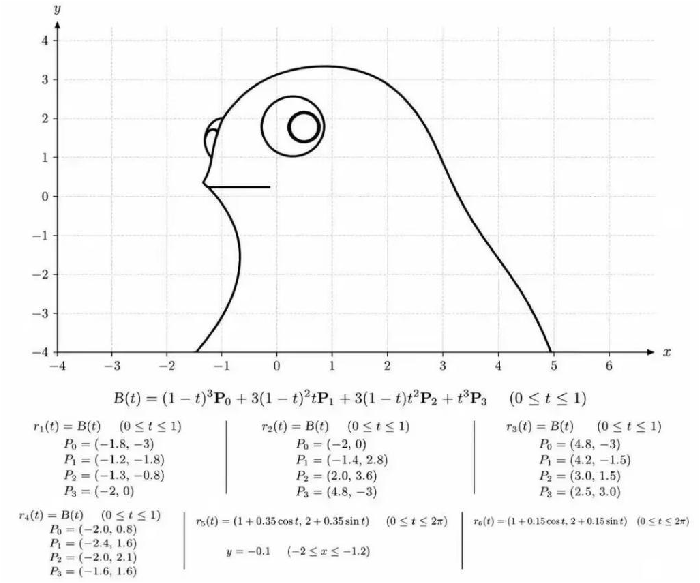
\includegraphics[width=285.43bp,height=0.76\textheight,keepaspectratio]{figures/chapter11/figure11_2.pdf}
  \renewcommand{\thefigure}{11.2}
  \caption{奶蛙曲线}
  \label{fig:11-2}
\end{figure}


\clearpage
% Source PDF page 50.
% !TEX root = ../../main.tex
\begin{figure}[H]
  \centering
  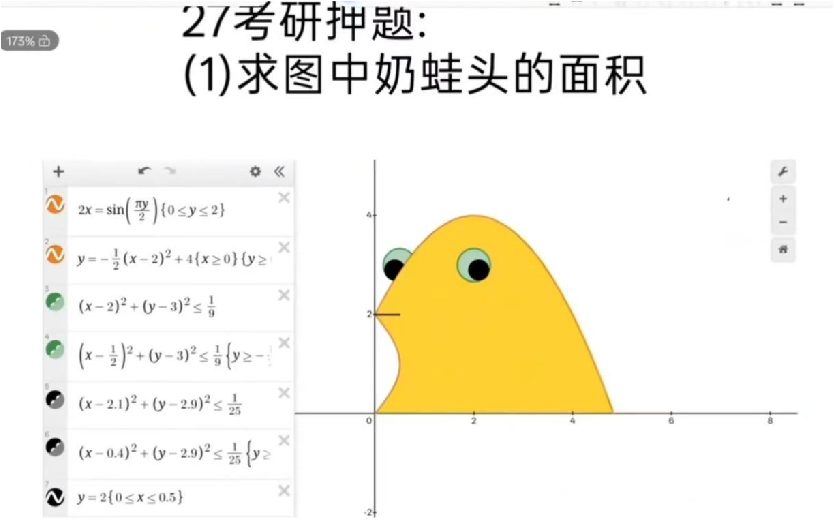
\includegraphics[width=340.41bp,height=0.76\textheight,keepaspectratio]{figures/chapter11/figure11_3.pdf}
  \renewcommand{\thefigure}{11.3}
  \caption{恶搞考研题：奶蛙头面积问题}
  \label{fig:11-3}
\end{figure}


\subsection{二、奶语言学}

由于日语中ないわ的罗马音为 na i wa（谐音奶蛙），因此一些耳朵尖的青年使用曾经在网上火过的“仙人指路”法，把一些歌曲中的ないわ圈出来并指向奶蛙，形成了非常搞笑的效果。~(见\figref{fig:11-4})

% !TEX root = ../../main.tex
\begin{figure}[H]
  \centering
  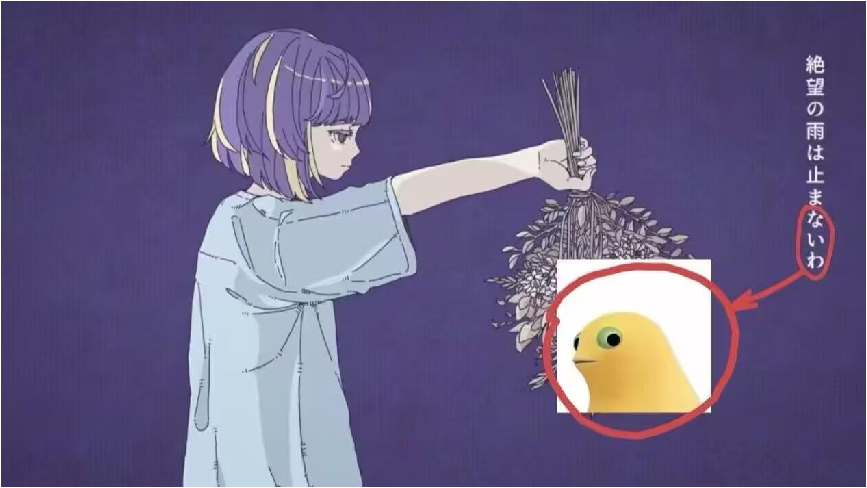
\includegraphics[width=353.77bp,height=0.76\textheight,keepaspectratio]{figures/chapter11/figure11_4.pdf}
  \renewcommand{\thefigure}{11.4}
  \caption{歌曲 phony 中的ないわ}
  \label{fig:11-4}
\end{figure}


\subsection{三、奶艺术学和奶历史学}

将梗糅合进入艺术和历史等通俗文科领域，以取得与现实大致相似却稍有不同的微妙效果，是互联网常见的一种做法。

而对比奶龙更接近于人形、拥有无穷无尽变种的奶蛙在这一点上明显有着巨大的优势。因此，奶蛙形成的奶艺术学和奶历史学拥有无比巨大的规模，给我们带来了一场视觉盛宴。~(见\figref{fig:11-5}, \figref{fig:11-7}, \figref{fig:11-8})

\clearpage
% Source PDF page 51.
% !TEX root = ../../main.tex
\begin{figure}[H]
  \centering
  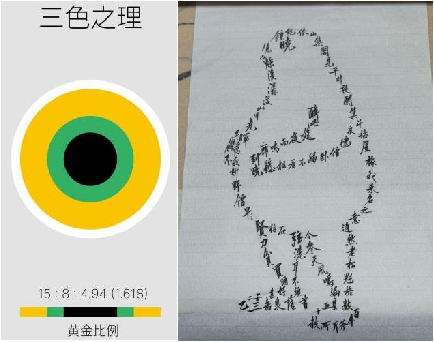
\includegraphics[width=176.9bp,height=0.76\textheight,keepaspectratio]{figures/chapter11/figure11_5.pdf}
  \renewcommand{\thefigure}{11.5}
  \caption{奶蛙黄金比（左）和由潇洒字体围成的奶蛙（右）}
  \label{fig:11-5}
\end{figure}


% !TEX root = ../../main.tex
\begin{figure}[H]
  \centering
  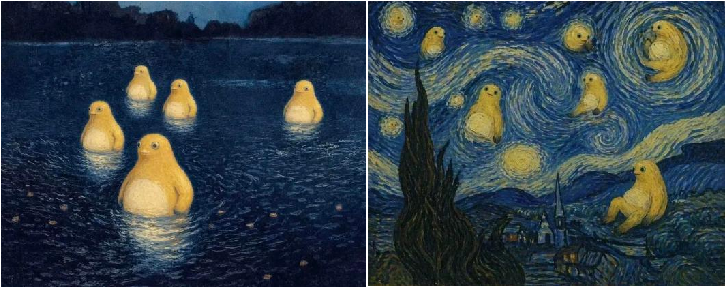
\includegraphics[width=296.24bp,height=0.76\textheight,keepaspectratio]{figures/chapter11/figure11_6.pdf}
  \renewcommand{\thefigure}{11.6}
  \caption{世界名画：河上的奶蛙（左）和奶空（右）}
  \label{fig:11-6}
\end{figure}


《河上的奶蛙》是对挪威著名画家弗里茨·索洛（Frits Thaulow）1880 年作品的模仿奶作，作品描绘了宁静河面上几只优雅的奶蛙，水面映照出周围景物的倒影，营造出神秘而安静的氛围。画面延续了索洛对水景的细腻刻画：深蓝色的水面通过丰富而流动的笔触表现出微妙的波纹变化，反射出环境的朦胧光影。奶蛙以柔和的暖黄色呈现，其圆润的体态在水中形成轻微的倒影与光晕，与周围环境自然融合。艺术家通过对光线的控制，使奶蛙周围的水面略显明亮，既强化了主体，又保持了整体画面的统一与和谐。作为 19 世纪挪威重要的风景画家之一，弗里茨·索洛以擅长描绘自然光线下的水面效果而著称。他的作品常通过细腻的观察与丰富的色彩变化，表现水流的动态与环境的静谧。在《河上的奶蛙》中，这种对水面质感与光影变化的表现依然得以保留，并通过新的形象转化，呈现出一种介于传统自然描绘与当代视觉符号之间的独特效果。~(见\figref{fig:11-6})

% !TEX root = ../../main.tex
\begin{figure}[H]
  \centering
  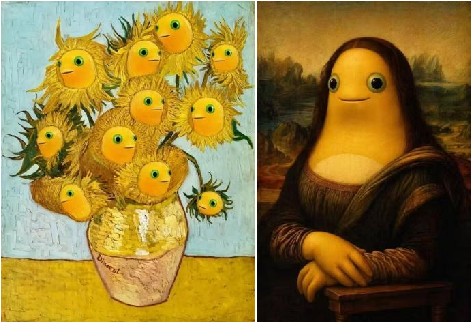
\includegraphics[width=192.41bp,height=0.76\textheight,keepaspectratio]{figures/chapter11/figure11_7.pdf}
  \renewcommand{\thefigure}{11.7}
  \caption{世界名画：向日奶（左）和蒙奶丽莎（右）}
  \label{fig:11-7}
\end{figure}


\clearpage
% Source PDF page 52.
% !TEX root = ../../main.tex
\begin{figure}[H]
  \centering
  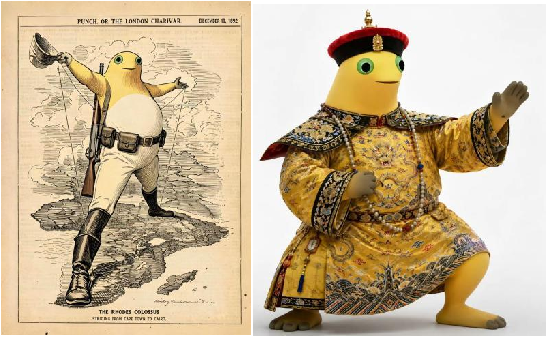
\includegraphics[width=223.31bp,height=0.76\textheight,keepaspectratio]{figures/chapter11/figure11_8.pdf}
  \renewcommand{\thefigure}{11.8}
  \caption{奶蛙在非洲的野心（左）和奶蛙帝国的安迪皇帝（右）}
  \label{fig:11-8}
\end{figure}


\subsection{四、奶烹饪技术学}

众所周知，奶龙的黄颜色和圆滚滚的形体，让人很自然地联想到黄桃罐头。因此，产生了奶龙尸块是黄桃罐头的说法。这一说法继承给了同样黄色、同样肚皮圆滚滚的奶蛙。~(见\figref{fig:11-9})

% !TEX root = ../../main.tex
\begin{figure}[H]
  \centering
  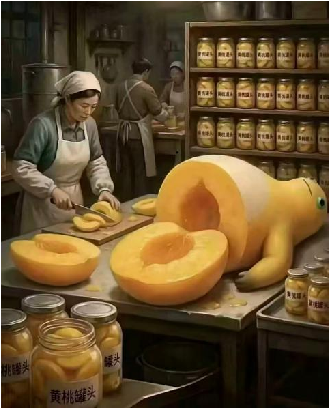
\includegraphics[width=134.78bp,height=0.76\textheight,keepaspectratio]{figures/chapter11/figure11_9.pdf}
  \renewcommand{\thefigure}{11.9}
  \caption{奶蛙被做成“黄桃罐头”}
  \label{fig:11-9}
\end{figure}


这一说法巧妙地给奶蛙加入了可食用的属性。由此，人们开始创作有关食物的奶蛙形象，甚至亲自动手做出吃的到的奶味食品。自此，奶烹饪技术学成为了一门颇为有趣的奶科学。~(见\figref{fig:11-10}, \figref{fig:11-11})

% !TEX root = ../../main.tex
\begin{figure}[H]
  \centering
  
\includegraphics[width=134.78bp,height=0.76\textheight,keepaspectratio]{figures/chapter11/figure11_10.pdf}
  \renewcommand{\thefigure}{11.10}
  \caption{奶蛙被做成“黄桃罐头”}
  \label{fig:11-10}
\end{figure}


\clearpage
% Source PDF page 53.
% !TEX root = ../../main.tex
\begin{figure}[H]
  \centering
  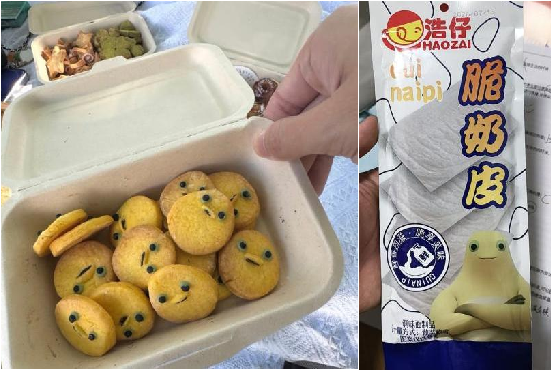
\includegraphics[width=225.15bp,height=0.76\textheight,keepaspectratio]{figures/chapter11/figure11_11.pdf}
  \renewcommand{\thefigure}{11.11}
  \caption{小红书某博主的手工奶蛋饼干（左）和一些食品商家推出的脆奶皮（右）}
  \label{fig:11-11}
\end{figure}


\subsection{五、奶哲学}

奶蛙一直在捧腹大笑，周而复始。因此，我们必须想象西西弗奶是幸福的。这就是奶哲学告诉我们的道理。奶哲学这一系中有名著《奶托邦》，能够启发我们对不同社会模式和生存方式的反思。我们这里引用几句：~(见\figref{fig:11-12})

奶托邦意为“根本没有的地方”。根本没有这样的地方！——《奶托邦》

我们一度怀疑自己来到了传说中的蜜与奶之地...“安迪！”他们看到我们，就突然抬起头，发出一种嘹亮的叫声。——《奶托邦》

% !TEX root = ../../main.tex
\begin{figure}[H]
  \centering
  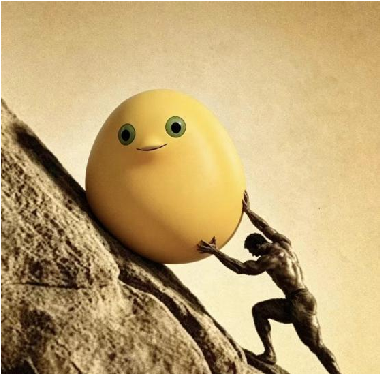
\includegraphics[width=155.38bp,height=0.76\textheight,keepaspectratio]{figures/chapter11/figure11_12.pdf}
  \renewcommand{\thefigure}{11.12}
  \caption{正在搬运奶蛋的西西弗奶}
  \label{fig:11-12}
\end{figure}


\subsection{六、奶政治学与奶法律学}

\textbf{【免责声明】}本节条文为架空内容，\textbf{不具有任何政治、法律效力，没有对现实中任何国家的政治制度和法律进行模仿、影射、亵渎。}不当改动本节内容可能引发不必要的风波，故本书编写组\textbf{不建议其他编写组对此节进行任何改动。若改编者私自在本节内塞入有关现实政治、法律私货进行反动宣传，并因此被抓获受到严厉法律处罚，本书不承担包括但不限于诱导、教唆犯罪等相关法律责任。}

在华科的龙蛙之争结束后，奶家人们意识到了需要一些特定称谓来形容一些影响奶蛙活动的不当行为。于是，一些奶家人开始使用被各种奶化了的罪名和一些俏皮调侃的“处罚”来模拟奶国法律处罚宣判时的可能情景，由此形成了奶法律学的雏形。

例如，如下的“剥夺大笑权利终身”就是奶国的最高惩罚之一。~(见\figref{fig:11-13})

\clearpage
% Source PDF page 54.
% !TEX root = ../../main.tex
\begin{figure}[H]
  \centering
  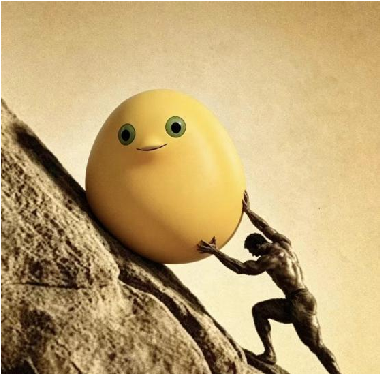
\includegraphics[width=155.38bp,height=0.76\textheight,keepaspectratio]{figures/chapter11/figure11_13.pdf}
  \renewcommand{\thefigure}{11.13}
  \caption{正在搬运奶蛋的西西弗奶}
  \label{fig:11-13}
\end{figure}


\subsection[七、奶工程学]{七、奶工程学~(见\figref{fig:11-14}, \figref{fig:11-15})}

% !TEX root = ../../main.tex
\begin{figure}[H]
  \centering
  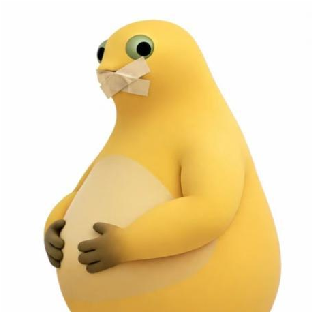
\includegraphics[width=281.55bp,height=0.76\textheight,keepaspectratio]{figures/chapter11/figure11_14.pdf}
  \renewcommand{\thefigure}{11.14}
  \caption{奶蛙模拟电路绘图}
  \label{fig:11-14}
\end{figure}


% !TEX root = ../../main.tex
\begin{figure}[H]
  \centering
  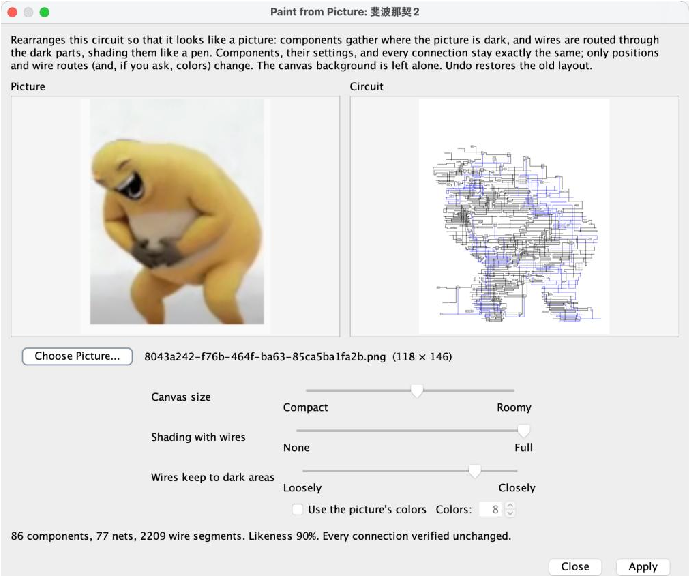
\includegraphics[width=281.55bp,height=0.76\textheight,keepaspectratio]{figures/chapter11/figure11_15.pdf}
  \renewcommand{\thefigure}{11.15}
  \caption{奶蛙模拟电路绘图}
  \label{fig:11-15}
\end{figure}


\clearpage
% Source PDF page 55.
\subsection[八、奶生物学和奶医学]{八、奶生物学和奶医学~(见\figref{fig:11-16})}

% !TEX root = ../../main.tex
\begin{figure}[H]
  \centering
  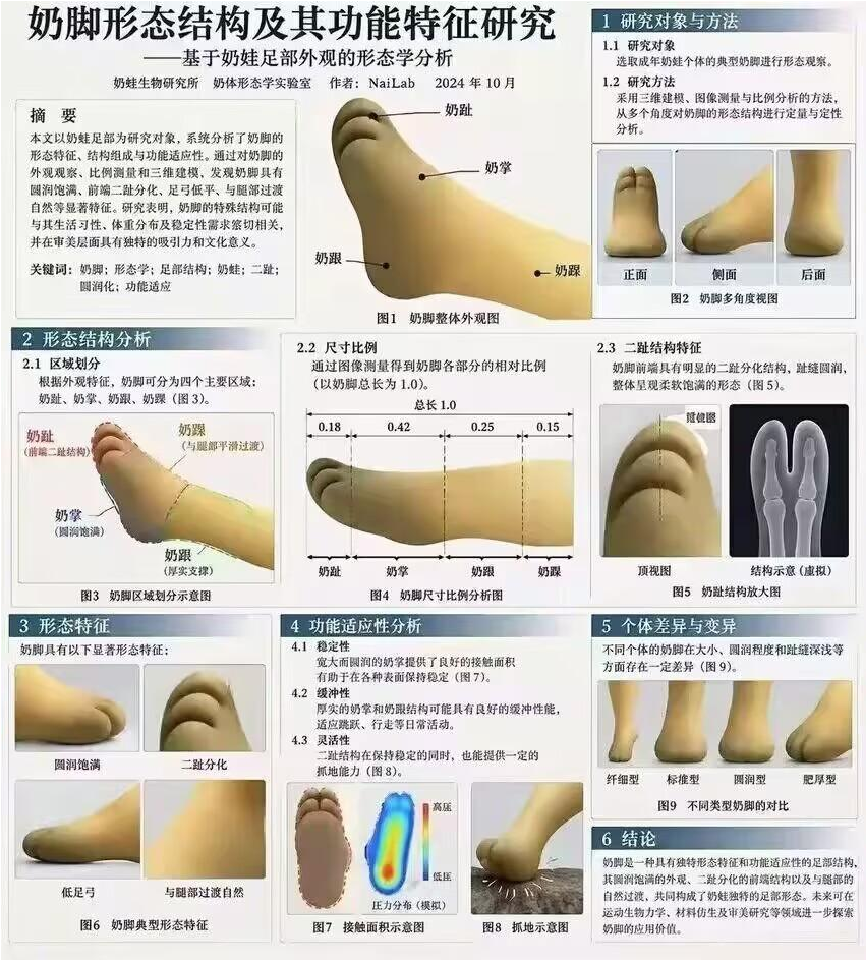
\includegraphics[width=273.19bp,height=0.76\textheight,keepaspectratio]{figures/chapter11/figure11_16.pdf}
  \renewcommand{\thefigure}{11.16}
  \caption{奶蛙户型设计（左）和掌握单片机力量的奶蛙（右）}
  \label{fig:11-16}
\end{figure}


\subsection{九、奶地理学}

“世界就是一个巨大的奶蛙。”这是奶地理学的真谛。~(见\figref{fig:11-17})

% !TEX root = ../../main.tex
\begin{figure}[H]
  \centering
  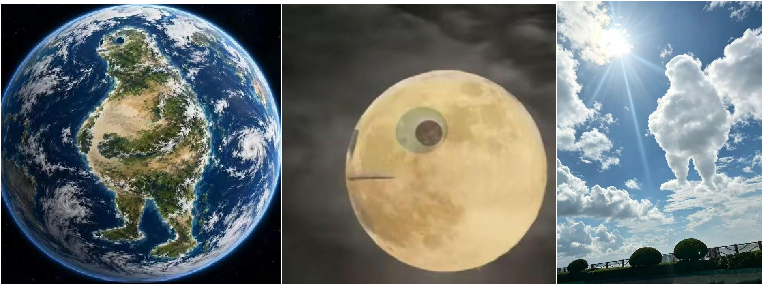
\includegraphics[width=311.13bp,height=0.76\textheight,keepaspectratio]{figures/chapter11/figure11_17.pdf}
  \renewcommand{\thefigure}{11.17}
  \caption{奶地球的古大陆（左）、奶月球（中）、奶云层（右）}
  \label{fig:11-17}
\end{figure}


\clearpage
% Source PDF page 56.
\subsection{十、奶体育运动学}

“你跑不过我你信吗？”这是奶雪峰牢师曾经说过的名言。虽然大家不愿意运动是正常的，但是，在学校和公司我们就练起来\textasciitilde{}~(见\figref{fig:11-18}, \figref{fig:11-19})

% !TEX root = ../../main.tex
\begin{figure}[H]
  \centering
  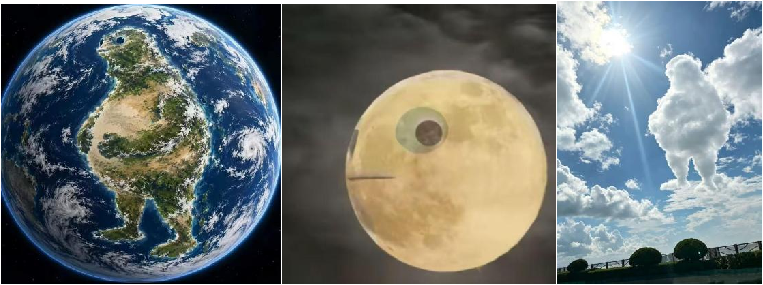
\includegraphics[width=311.13bp,height=0.76\textheight,keepaspectratio]{figures/chapter11/figure11_18.pdf}
  \renewcommand{\thefigure}{11.18}
  \caption{奶地球的古大陆（左）、正在思考要不要引发潮汐的奶月球（中）、奶云层（右）}
  \label{fig:11-18}
\end{figure}


% !TEX root = ../../main.tex
\begin{figure}[H]
  \centering
  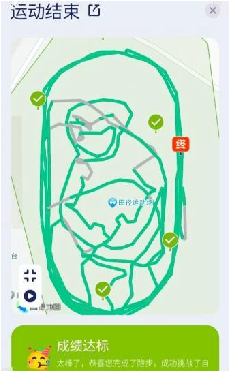
\includegraphics[width=267.17bp,height=0.76\textheight,keepaspectratio]{figures/chapter11/figure11_19.pdf}
  \renewcommand{\thefigure}{11.19}
  \caption{正在打乒乓球的奶蛙（？！赶紧上？！）}
  \label{fig:11-19}
\end{figure}


\subsection{十一、奶考古学}

根本就没有这样的文物！（你只是怕了）~(见\figref{fig:11-20})

% !TEX root = ../../main.tex
\begin{figure}[H]
  \centering
  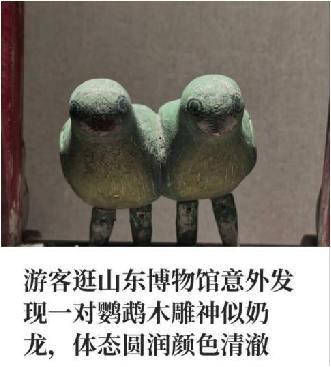
\includegraphics[width=267.17bp,height=0.76\textheight,keepaspectratio]{figures/chapter11/figure11_20.pdf}
  \renewcommand{\thefigure}{11.20}
  \caption{正在打乒乓球的奶蛙（？！赶紧上？！）}
  \label{fig:11-20}
\end{figure}


\clearpage
% Source PDF page 57.
\subsection{十二、奶游戏娱乐学}

在奶国杀里面，奶蛙的强度究竟阴间不阴间？

我们脑杀推测，奶蛙在军八里面的强度绝对不高，但是娱乐性节目效果极强。奶蛙只有三滴血，相当于一个脆皮白板将，但是技能\textbf{【大笑】}可以像病毒一样蔓延开来，把所有人都慢慢变成白板将，就算被打下场也仍然影响着全局。这种特性让奶蛙就算是顶阴局也能有一席之地，只不过选出来不是为了赢，而是为了玩。当所有人的技能都变成\textbf{【大笑】}，胜负根本已经不重要了。这张卡完美契合奶蛙大笑的传染力，设计给到夯。~(见\figref{fig:11-21})

% !TEX root = ../../main.tex
\begin{figure}[H]
  \centering
  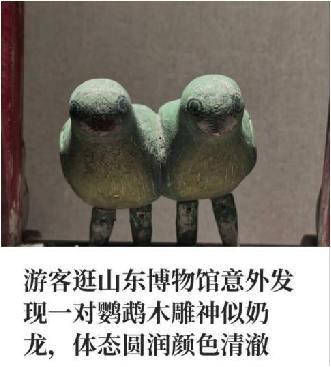
\includegraphics[width=173.74bp,height=0.76\textheight,keepaspectratio]{figures/chapter11/figure11_21.pdf}
  \renewcommand{\thefigure}{11.21}
  \caption{奶国杀中奶蛙的武将牌（作者：阿茶妹妹）}
  \label{fig:11-21}
\end{figure}

